%%%%%%%%%%%%%%%%%%%%%%%%%%%%%%%%%%%%%%%%%
% Stylish Article
% LaTeX Template
% Version 2.0 (13/4/14)
%
% This template has been downloaded from:
% http://www.LaTeXTemplates.com
%
% Original author:
% Mathias Legrand (legrand.mathias@gmail.com)
%
% License:
% CC BY-NC-SA 3.0 (http://creativecommons.org/licenses/by-nc-sa/3.0/)
%
%%%%%%%%%%%%%%%%%%%%%%%%%%%%%%%%%%%%%%%%%

%----------------------------------------------------------------------------------------
%	PACKAGES AND OTHER DOCUMENT CONFIGURATIONS
%----------------------------------------------------------------------------------------

\documentclass[fleqn,10pt]{SelfArx} % Document font size and equations flushed left


%----------------------------------------------------------------------------------------
%	Source Code Listings
%----------------------------------------------------------------------------------------
\usepackage{listings}
\usepackage{xcolor}
\definecolor{darkgreen}{rgb}{0.0, 0.2, 0.13}
\definecolor{ao}{rgb}{0.0, 0.5, 0.0}
\lstdefinestyle{sharpc}{language=[Sharp]C, frame=single}
\lstset{% general command to set parameter(s)
basicstyle=\small, % print whole listing small
keywordstyle=\color{blue}\bfseries,
% underlined bold black keywords
commentstyle=\small\color{ao}, % white comments
stringstyle=\ttfamily, % typewriter type for strings
columns=fullflexible, % keeps the comments from exploding
showstringspaces=false} % no special string spaces


% Algorithms package
\usepackage{fancybox}
\usepackage{algorithm}
\usepackage{caption}
\usepackage{algorithmic}
\usepackage{bm}

\usepackage{breqn}

%----------------------------------------------------------------------------------------
%	COLUMNS
%----------------------------------------------------------------------------------------

\setlength{\columnsep}{0.55cm} % Distance between the two columns of text
\setlength{\fboxrule}{0.75pt} % Width of the border around the abstract

%----------------------------------------------------------------------------------------
%	COLORS
%----------------------------------------------------------------------------------------

\definecolor{color1}{RGB}{0,0,90} % Color of the article title and sections
\definecolor{color2}{RGB}{0,20,20} % Color of the boxes behind the abstract and headings

%----------------------------------------------------------------------------------------
%	HYPERLINKS
%----------------------------------------------------------------------------------------

\usepackage{hyperref} % Required for hyperlinks
\hypersetup{hidelinks,colorlinks,breaklinks=true,urlcolor=color2,citecolor=color1,linkcolor=color1,bookmarksopen=false,pdftitle={Title},pdfauthor={Author}}

%----------------------------------------------------------------------------------------
%	ARTICLE INFORMATION
%----------------------------------------------------------------------------------------

\JournalInfo{PBEP \#3, 2015} % Journal information
\Archive{PBEP Series} % Additional notes (e.g. copyright, DOI, review/research article)

\PaperTitle{PacBio Enhancement Proposal \#3 \\{\large Implementing a probability based scoring model for CCS}} % Article title

\Authors{Nigel Delaney and David Alexander} % Authors

\Keywords{} % Keywords - if you don't want any simply remove all the text between the curly brackets
\newcommand{\keywordname}{Keywords} % Defines the keywords heading name

%----------------------------------------------------------------------------------------
%	ABSTRACT
%----------------------------------------------------------------------------------------

\Abstract{ The current PacBio CCS scoring model does not work in probability space, resulting in several oddities and inefficiencies.  This proposal presents a new scoring scheme that, conditioned on QV scores associated with a read, calculates the probability that the read could have generated the derived template by integrating over all possible paths of insertions, deletions, mismatches and matches between the read and the template. }

%----------------------------------------------------------------------------------------

\begin{document}

\flushbottom % Makes all text pages the same height

\maketitle % Print the title and abstract box

\tableofcontents % Print the contents section

\thispagestyle{empty} % Removes page numbering from the first page

%----------------------------------------------------------------------------------------
%	ARTICLE CONTENTS
%----------------------------------------------------------------------------------------

\section{Introduction} % The \section*{} command stops section numbering


There is a long standing tradition in bioinformatics of generating alignments between sequences according to a dynamic programming method that scores alignments according to a fixed set of parameters for insertions, deletions, mismatches and matches.  More sophisticated frameworks treat the alignment problem using a probabilistic modeling framework, such as a Paired HMM model, in which there is a defined generative model with transition probabilities between insertion, deletion and match states.  It has been shown that when considering the optimal alignment, there is a direct correspondence between the probabilistic framework and the standard affine scoring dynamic programming method.\footnote{See the section \textit{The most probable path is the optimal FSA alignment} on page 82 in the book \textit{Biological Sequence Analysis} by Durbin et. al}

Using a probabilistic framework has numerous advantages compared to using a fixed scoring scheme.  Questions such as how much evidence is there for one alignment as compared to another are directly answered by comparing probabilities.  Additionally all the tools and historical research concerning probabilistic modeling become available, guiding the choices of optimization methods and offering asymptotic guarantees about their accuracy.  Finally, in the context of DNA sequencing probabilistic frameworks allow us to naturally integrate over all the ways a particular read could be generated from a particular template.

The PacBio analysis which generates consensus sequences does not currently use a probabilistic framework, a possibly glaring omission since there is a left-right HMM generative model believed to govern how PacBio reads are generated.\footnote{See the EDNA documentation for a discussion of this model.}  The central reason for this is that most probabilistic models use fixed parameters for transitions between states, while in practice there are often covariates associated with the bases of an emitted read that indicate how much certainty we have that they are a true representation of the template.

These covariates, typically condensed into QV values, are not easily incorporated into the PacBio probabilistic framework for how reads are generated, and so the statistical method of estimating models and parameters is abandoned in favor of a scoring scheme that rhymes with, though does not actually represent, a probability model.  Trouble quickly follows.  As examples of the difficulties presented by QV scores, consider how an insertion of size 2 is assessed from a probability perspective in the context of QV values, or how the probability of a deletion event, which is in many ways an attribute of the template, is instead assigned to read bases.

This proposal intends to create a framework for PacBio consensus scoring that represents a true probability model.  It will do this by making one central conceit, which is to invert the relationship between the read and the template.  Although we normally think of the read as being a noisy signal of the template and conceive of a generative model for $P(R|T)$, we will instead consider the generative model as the read giving rise to templates, in other words we will consider $P(T|R)$.  In doing so we will treat the read and it's associate QV values as fixed parameters, and given several such reads will find the template with the highest probability of occurring across a set of reads.  Although counterintuitive, once framed this way, we are easily able to incorporate the probabilities given by QV values and work in a probabilistic way.  This framework also allows us to cleanly separate the domains of primary and secondary analysis, with the transition between the two demarcated by the paradigm shift  $P(R|T) \rightarrow P(T|R) $ and the concurrent generation of the respective QV values as probabilities of certain events (which can be framed as maximizing the fixed parameters given the observed template). 



%------------------------------------------------

\section{The New Scoring Model and Associated QVs}

Table 1 shows the QV values that will go into the new scoring framework and what each will mean.  Note that, although in a standard context we refer to``deletions" as positions in an alignment where the template has a base but there is no base in the read, because we now view the read as the `reference', the labeling of insertions and deletions has been reversed.

\begin{table*}[bt]
\caption{Table of QV Meanings}
\centering
    \begin{tabular}{| l | p{7cm} | c | c |  }
    \toprule
    \hline
    \textbf{QV Value} &  \textbf{Represents the probability of:} &  \textbf{Notation for probability} &  \textbf{Analogous Edna move}  \\ \hline \hline
    Insertion Different & an insertion prior to this base of a different base than itself. & $p_{id}$  & Dark / null \\ \hline
    Insertion Same & an insertion prior to this base of the same base as itself.& $p_{is}$ & Merge \\ \hline
    Deletion Different & a deletion prior to this base of a different base than itself. & $p_{dd}$  & Stick \\ \hline
    Deletion Same & a deletion prior to this base of the same base as itself. & $p_{ds}$  & Branch \\ \hline
    Substitution & this base being emitted correctly conditioned on it being emitted & $p_{s}$  &  Misclassified \\ \hline
    \bottomrule
    \end{tabular}
\end{table*}





\subsection{ Calculating $\mathbf{P(T|R)}$} 

The inputs are a read of length, J, and a template of length I.  Each base in the read also has an associated QV values given by Table 1.   The algorithm proceeds by recursively populating a matrix and returning the bottom right value as described next.  In describing the algorithm and to account for offsetting, in what follows read and template positions are 1-based indexed, while positions in the matrix that are filled are referred to by 0-based indexes. 


\begin{algorithm}
\caption*{\textbf{Probability Calculation Algorithm}}
\label{calcScore}
\begin{algorithmic}[h]
\FOR{$j=1$ to J}
\FOR{$i=1$ to I}
\IF{ $i =0\ \& j =0 $}
\STATE $A[i,j] \leftarrow 0$
\ELSE
\STATE \[
	A[i,j]  \leftarrow \text{summed}
\begin{cases}
	\text{Match Probability} \\
	\text{Insertion Probability} \\
	\text{Deletion Probability} \\
   	\end{cases}
\]
\ENDIF	
\ENDFOR
\ENDFOR
\RETURN $A[I,J]$
\end{algorithmic}
\end{algorithm}





\subsection{Recursion steps}
After the matrix is initialized, each element in the matrix is recursively populated with the logarithm of the probability of an alignments ending at $i,j$ by examining the available moves, either an insertion, deletion or match.  If a particular step cannot be calculated because it is too close to the edge, it is skipped.  Each possible move is described next.  Top row and first column are initialized as deletions or insertions of the relevant length.  Note that in practice, the elements are stored as log probabilities, but are described as actual probabilities here to simplify the description.






\subsubsection{\textbf{Match}}


%\[
\begin{dmath}
\text{Match Probability} = \\
	 \alpha_{i-1,j-1}  \times  (1-p_{id}+p_{is}+p_{dd}+p_{ds})  \times 
	 \begin{cases}
							 \ (1-p_{s}) & \text{if }  R_{j} = T_{i} \\
							 \frac{1}{3} \times p_{s}  & \text{if }  R_{j}  \neq T_{i} 
							 \end{cases}
\end{dmath}
%\]

\begin{figure}[ht] %% The [h] means place the figure about here.
	\includegraphics[width=\linewidth]{Match}
		\caption{The calculation of the match score.  The upper element is added to an amount determined by the comparison of the bases shown.}
\end{figure}

This is simply the probability that a match event occurred (rather than an insertion or deletion), plus the appropriate emmission probability for the base (with a uniform probability,  $\frac{1}{3}$, for each possible incorrect base).

\subsubsection{\textbf{Insertion}}


\begin{dmath}
\text{Insertion Probability} = \\
	\alpha_{i-1,j}  \times 
	\begin{cases}
		p_{is_{j+1}}  & \text{if }  T_{i} = R_{j+1} \\
		p_{id_{j+1}} & \text{if }  T_{i}  \neq R_{j+1} 
	\end{cases}
\end{dmath}

\begin{figure}[ht] %% The [h] means place the figure here.
	\includegraphics[width=\linewidth]{Insertion}
		\caption{The calculation of the insertion value.  The upper diagonal element is added to an amount determined by the comparison of the bases shown.}
\end{figure}


This insertion score differs from what is typical.  It is designed to account for two separate events.  First, is designed to account for the possibility that two bases were read simultaneously as one base (presumably because the enzyme acquired the next base before a break in the signal intensity was observed, and if this was the same base, this could be interpreted as one merged pulse).
 
\subsubsection{\textbf{Deletion}}

\begin{figure}[ht] %% The [h] means place the figure about here.
	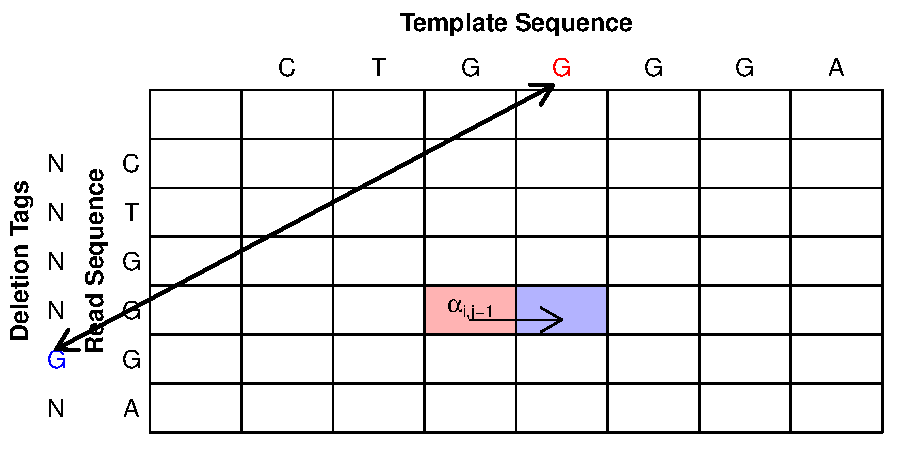
\includegraphics[width=\linewidth]{Deletion}
		\caption{The calculation of the deletion score.  The left matrix element is added to an amount determined by the comparison of the bases shown.}				
\end{figure}

\begin{dmath}
	\text{Deletion Probability} = \alpha_{i,j-1}  \\
	\times  \begin{cases}
				p_{ds_{j+1}}  & \text{if }  \text{R}_{j} = R_{j+1} \\
				p_{dd_{j+1}} & \text{if }  \text{R}_{j} \neq R_{j+1} 
				\end{cases}
\end{dmath}



The deletion probability, like the insertion probability, has two different values, and as before this is motivated by the underlying process determining how PacBio data is generated.  For PacBio data, there is a ``branching" process that occurs during nucleotide incorporation in which the polymerase may begin to incorporate a base and hold it long enough for the base to be detected in the sequencer before eventually releasing it after failing to complete the incorporation reaction.  In the event of a true branch, the inserted (or in our framework deleted) base should thus match the next template base.  Also as before, the observation could also have been caused by a non-branch event, namely a stick where the base happens to match, and so the QV value used is intended to encompass both a branch and non-branch event leading to this base being emitted.


%------------------------------------------------



\section{Conclusion}

Statistical models should be motivated by the underlying processes that generate the data, but inevitably must make concessions to bias versus variance trade-offs that will govern if in practice the model can perform adequately for the purpose it is designed for.

Our current CCS consensus model is poor largely because it examined this trade-off and sort of lost at both bias and variance.  Variance in parameter estimates, such as the QV recalibration, is introduced because the same observed error, such as a deletion in a homopolymer, could be explained by multiple different events but by using Viterbi scoring only one of these could be considered, leading to multiple modes in the optimization.  Similarly, bias is introduced because in addition to the hard-coded values everywhere, the model does not adequately capture the generative process in which multiple events can lead to the same outcome, forcing it to make artificial trade-offs required when one possibility must represent all possibilities.

This new model is simpler and more unified.  Although considering $P(T|R)$ seems unusual, taking this plunge immediately allows us to maximize the probability of the template sequence given the reads, and provides a statistical framework with which to compare possible consensus sequences.  It can also be seen as an approximation of the Bayes corollarly, which we need to use if we maintained the model for $P(R|T)$ such that we would need to calculate:

\begin{dmath}
P(R|T) = \frac{P(T|R) \cdot P(R)}{P(T)}
\end{dmath}

Although this equation is the fundamentally correct model for primary to optimize the raw read accuracy, the denominator, $P(T)$ is irrelevant if we use a uniform prior over templates, and the probability of the read and it's associated QV values, $P(R)$, is neither defined and almost certainly would be challenging to calculate even if we could define it.  The calculation of $P(R)$ is a fundamental problem that makes modeling difficult.  In contrast, this framework effectively sets $P(R) = 1$ and can be seen as a very strong prior on the observed data (and after all, that read already has been observed to have occurred).  

  Additionally, though the generative model itself has quite changed, the intuition governing the model has been carried over, with every type of move in the generative Edna model having a corresponding QV value and scoring mechanism in the algorithm.  However, nuisances edge cases, such as Deletion Tags and how the separate  `Knight's move' to represent a deletion in a homopolymer context have been excised.   In the later case, the underlying intuition has still been preserved in scoring that captures the branch or merge moves respectively, we have simply replace multiple ways to score these observations with a single one.

Finally, it is worth commenting on how to calculate the QV models in this new framework.  This will be the subject of another write-up, but at present I think it suffices to say that while QV scores are traditionally calculated marginally (that is without any knowledge of the other QVs or there relationship to the true template), one hundred years of statistical literature says that with a unified model it is best to jointly estimate parameters.  In this regard, given any framework we can directly maximize $P(T|R)$, and green pastures likely await there.


    
  

%----------------------------------------------------------------------------------------

\end{document}